%% Module 2 beamer/knitr slides
%% Biostatistics in Practice workshop, January 2014
%% Nicholas Reich: nick [at] schoolph.umass.edu


\documentclass[table]{beamer}\usepackage[]{graphicx}\usepackage[]{color}
% maxwidth is the original width if it is less than linewidth
% otherwise use linewidth (to make sure the graphics do not exceed the margin)
\makeatletter
\def\maxwidth{ %
  \ifdim\Gin@nat@width>\linewidth
    \linewidth
  \else
    \Gin@nat@width
  \fi
}
\makeatother

\definecolor{fgcolor}{rgb}{0.345, 0.345, 0.345}
\newcommand{\hlnum}[1]{\textcolor[rgb]{0.686,0.059,0.569}{#1}}%
\newcommand{\hlstr}[1]{\textcolor[rgb]{0.192,0.494,0.8}{#1}}%
\newcommand{\hlcom}[1]{\textcolor[rgb]{0.678,0.584,0.686}{\textit{#1}}}%
\newcommand{\hlopt}[1]{\textcolor[rgb]{0,0,0}{#1}}%
\newcommand{\hlstd}[1]{\textcolor[rgb]{0.345,0.345,0.345}{#1}}%
\newcommand{\hlkwa}[1]{\textcolor[rgb]{0.161,0.373,0.58}{\textbf{#1}}}%
\newcommand{\hlkwb}[1]{\textcolor[rgb]{0.69,0.353,0.396}{#1}}%
\newcommand{\hlkwc}[1]{\textcolor[rgb]{0.333,0.667,0.333}{#1}}%
\newcommand{\hlkwd}[1]{\textcolor[rgb]{0.737,0.353,0.396}{\textbf{#1}}}%
\let\hlipl\hlkwb

\usepackage{framed}
\makeatletter
\newenvironment{kframe}{%
 \def\at@end@of@kframe{}%
 \ifinner\ifhmode%
  \def\at@end@of@kframe{\end{minipage}}%
  \begin{minipage}{\columnwidth}%
 \fi\fi%
 \def\FrameCommand##1{\hskip\@totalleftmargin \hskip-\fboxsep
 \colorbox{shadecolor}{##1}\hskip-\fboxsep
     % There is no \\@totalrightmargin, so:
     \hskip-\linewidth \hskip-\@totalleftmargin \hskip\columnwidth}%
 \MakeFramed {\advance\hsize-\width
   \@totalleftmargin\z@ \linewidth\hsize
   \@setminipage}}%
 {\par\unskip\endMakeFramed%
 \at@end@of@kframe}
\makeatother

\definecolor{shadecolor}{rgb}{.97, .97, .97}
\definecolor{messagecolor}{rgb}{0, 0, 0}
\definecolor{warningcolor}{rgb}{1, 0, 1}
\definecolor{errorcolor}{rgb}{1, 0, 0}
\newenvironment{knitrout}{}{} % an empty environment to be redefined in TeX

\usepackage{alltt}


%       ************************************************
%       **        LaTeX preamble to be used with all 
%	**        statsTeachR labs/handouts.
%
%	Author: Nicholas G Reich
%	Last modified: 14 January 2014
%	************************************************

% \documentclass[table]{beamer}

%	Set theme (a nice plain one)
\usetheme{Malmoe}

%	Use named colors, set main color of theme
%		to match Web site color:
\definecolor{MainColor}{RGB}{10, 74, 109}
\colorlet{MainColorMedium}{MainColor!50}
\colorlet{MainColorLight}{MainColor!20}
\usecolortheme[named=MainColor]{structure} 

%	For tables
%[dvipsnames] [table]
\usepackage{xcolor}

%% calling tabu.sty, assuming a particular directory structure
\usepackage{../../slide-includes/tabu}	% Even fancier than tabulary
\usepackage{multirow}

%	Just for the degree symbol
\usepackage{textcomp}

%	Get rid of footline (page, author, etc. on each slide)
\setbeamertemplate{footline}{}
%	Get rid of navigation buttons
\setbeamertemplate{navigation symbols}{}

%	Make footnotes not ugly
\usepackage{hanging}
\setbeamertemplate{footnote}{\raggedright\hangpara{1em}{1}\makebox[1em][l]{\insertfootnotemark}\footnotesize\insertfootnotetext\par}

%	Text style for code snippets inline in text:
\newcommand{\codeInline}[1]{\texttt{#1}}

%	Text style for emphasis stronger than \emph:
%		(Note, this doesn't toggle the way \emph does.
%			(Note, this can be done, didn't seem worth the trouble.))
\newcommand{\strong}[1]{{\bfseries{#1}}}


%        ******	Define title page	**********************
\setbeamertemplate{title page}{
	{\color{MainColor}
	% There must be a better way than this -vspace at
	%	 the top and bottom of the page to reduce the 
	%	 bottom margin, but I can't find one that works.
	\vspace{-6em}

% 	% Go to a lot of trouble to get the title in a
% 	%	nice box, since customizing a beamer block
% 	%	does not entirely work here (I don't know why)
	\newlength{\titleBoxWidth}
	\setlength{\titleBoxWidth}{\textwidth}
	\addtolength{\titleBoxWidth}{-2.0em}
	\setlength{\fboxsep}{1.0em}
	\setlength{\fboxrule}{0pt}
	\fcolorbox{MainColor!25}{MainColor!25}{
		\parbox{\titleBoxWidth}{
			\raggedright
			\LARGE\textbf{\inserttitle}
		}	% end parbox
	}	% end fcolorbox

	\vfill
	\small{Author: \insertauthor}
	\vspace{\baselineskip}

	\small{\Course}

	\small{\Instructor}
	\vspace{\baselineskip}

	%\small{\emph{This material is part of the \strong{statsTeachR} project}}

	\vspace{0.33\baselineskip}\scriptsize{\emph{\LicenseText}}


		\vspace{-15em}

	}	% end color
	\clearpage
}	% end define title page

%        The following variables are assumed by the standard preamble:
%	Global variable containing module name:
\title{Introduction to Logistic Regression}
%	Global variable containing module shortname:
%		(Currently unused, may be used in future.)
\newcommand{\ModuleShortname}{MLR}
%	Global variable containing author name:
\author{Nicholas G Reich}
%	Global variable containing text of license terms:
\newcommand{\LicenseText}{Made available under the Creative Commons Attribution-ShareAlike 3.0 Unported License: http://creativecommons.org/licenses/by-sa/3.0/deed.en\_US }
%	Instructor: optional, can leave blank.
%		Recommended format: {Instructor: Jane Doe}
\newcommand{\Instructor}{}
%	Course: optional, can leave blank.
%		Recommended format: {Course: Biostatistics 101}
\newcommand{\Course}{}

\input{../../slide-includes/shortcuts}
\usepackage{bbm}
\hypersetup{colorlinks=TRUE, urlcolor=blue}

%%%%%%%% IMPORTANT -- MUST HAVE [fragile] for some/all frames chunks to have output work correctly.
\IfFileExists{upquote.sty}{\usepackage{upquote}}{}
\begin{document}




\begin{frame}[plain]
        \titlepage
\end{frame}




%%%%%%%%%%%%%%%%%%%%%%%%%%%%%%%%%%%%%%%%%%

\begin{frame}{Today's Lecture}


\bi
	\myitem Logistic regression
\ei

[Note: more on logistic regression can be found in Kaplan, Chapter 16 and the OpenIntro Statistics textbook, Chapter 8. These slides are based, in part, on the slides from OpenIntro.]

\end{frame}

%%%%%%%%%%%%%%%%%%%%%%%%%%%%%%%%%%%%

\begin{frame}
\frametitle{Regression so far ...}
    
At this point we have covered:

{\small
\begin{itemize}
\item Simple linear regression
\begin{itemize}
\item Relationship between numerical response and a numerical or categorical predictor
\end{itemize}
\item Multiple regression
\begin{itemize}
\item Relationship between numerical response and multiple numerical and/or categorical predictors
\end{itemize}
\end{itemize}
}


What we haven't covered is what to do when the response is not continuous (i.e. categorical, count data, etc.)


\end{frame}


%%%%%%%%%%%%%%%%%%%%%%%%%%%%%%%%%%%

\begin{frame}[fragile]{Refresher: regression estimates the average response}

In linear regression, when y is a continuous variable, our model estimates for us the average $y$, $\hat y$, value for a particular value of $x$.

\begin{knitrout}\scriptsize
\definecolor{shadecolor}{rgb}{0.969, 0.969, 0.969}\color{fgcolor}

{\centering \includegraphics[width=\maxwidth]{figure/beamer-unnamed-chunk-1-1} 

}



\end{knitrout}

\end{frame}

%%%%%%%%%%%%%%%%%%%%%%%%%%%%%%%%%%%

\begin{frame}[fragile]{Refresher: regression estimates the average response}

When y is a binary outcome variable, regression models can still estimate for us the average $y$, $\hat y$, but now it represents something different: the probability that $y = 1$, or $P(Y=1)$.

\begin{knitrout}\scriptsize
\definecolor{shadecolor}{rgb}{0.969, 0.969, 0.969}\color{fgcolor}

{\centering 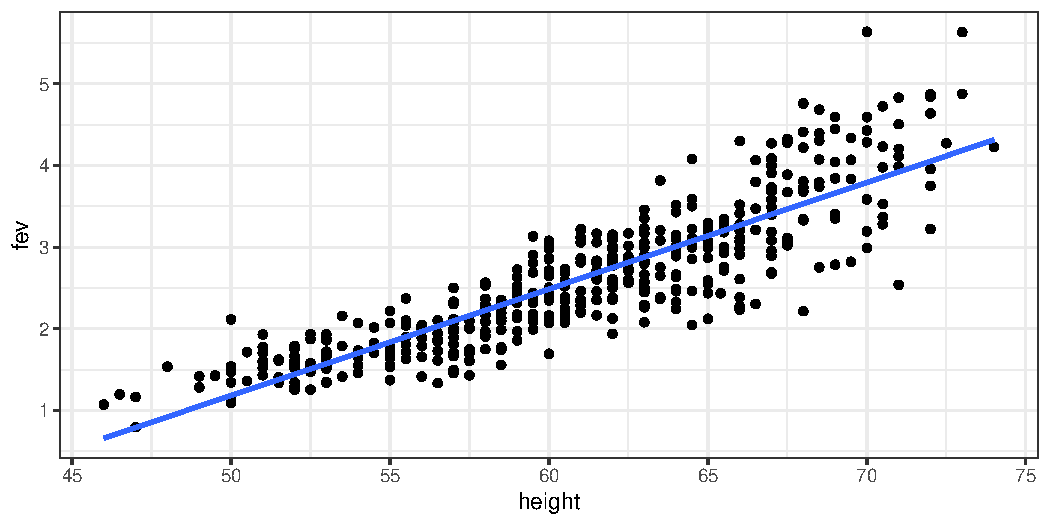
\includegraphics[width=\maxwidth]{figure/beamer-unnamed-chunk-2-1} 

}



\end{knitrout}

\end{frame}

%%%%%%%%%%%%%%%%%%%%%%%%%%%%%%%%%%%


\begin{frame}
\frametitle{Example - Birdkeeping and Lung Cancer}

A 1972 - 1981 health survey in The Hague, Netherlands, discovered an association between keeping pet birds and increased risk of lung cancer. To investigate birdkeeping as a risk factor, researchers conducted a case-control study of patients in 1985 at four hospitals in The Hague (population 450,000). They identified 49 cases of lung cancer among the patients who were registered with a general practice, who were age 65 or younger and who had resided in the city since 1965. They also selected 98 controls from a population of residents having the same general age structure.


\vfill

{\tiny \textit{Ramsey, F.L. and Schafer, D.W. (2002). The Statistical Sleuth: A Course in Methods of Data Analysis (2nd ed)}}
\end{frame}

%%%%%%%%%%%%%%%%%%%%%%%%%%%%%%%%%%%

\begin{frame}[fragile]{Example - Birdkeeping and Lung Cancer - Data}

{\small
\begin{knitrout}\scriptsize
\definecolor{shadecolor}{rgb}{0.969, 0.969, 0.969}\color{fgcolor}\begin{kframe}
\begin{alltt}
\hlkwd{library}\hlstd{(Sleuth3)}
\hlstd{birds} \hlkwb{=} \hlstd{case2002}
\hlkwd{head}\hlstd{(birds)}
\end{alltt}
\begin{verbatim}
##           LC   FM   SS     BK AG YR CD
## 1 LungCancer Male  Low   Bird 37 19 12
## 2 LungCancer Male  Low   Bird 41 22 15
## 3 LungCancer Male High NoBird 43 19 15
## 4 LungCancer Male  Low   Bird 46 24 15
## 5 LungCancer Male  Low   Bird 49 31 20
## 6 LungCancer Male High NoBird 51 24 15
\end{verbatim}
\end{kframe}
\end{knitrout}
}

%~\\

{\tiny
\begin{center}
\begin{tabular}{ll}
LC & Whether subject has lung cancer \\
FM & Sex of subject \\
SS & Socioeconomic status \\
BK & Indicator for birdkeeping \\
AG & Age of subject (years) \\
YR & Years of smoking prior to diagnosis or examination \\
CD & Average rate of smoking (cigarettes per day)
\end{tabular}
\end{center}
}

\tiny{NoCancer is the reference response (0 or failure), LungCancer is the non-reference response (1 or success) - this matters for interpretation.}

\end{frame}





%%%%%%%%%%%%%%%%%%%%%%%%%%%%%%%%%%%

\begin{frame}[fragile]{Example - Birdkeeping and Lung Cancer - Data}

What types of associations do you expect to see between the predictors below and lung cancer? Might you expect any interactions to be present?

{
\begin{center}
\begin{tabular}{ll}
LC & Whether subject has lung cancer \\
FM & Sex of subject \\
SS & Socioeconomic status \\
BK & Indicator for birdkeeping \\
AG & Age of subject (years) \\
YR & Years of smoking prior to diagnosis or examination \\
CD & Average rate of smoking (cigarettes per day)
\end{tabular}
\end{center}
}

\end{frame}



%%%%%%%%%%%%%%%%%%%%%%%%%%%%%%%%%%%


\begin{frame}[fragile]{Interpreting linear regressions of binary data}

We can use linear regression for binary data, and for {\em very simple models} it gives reasonable and interpretable output.

$$ \hat LC_i = \beta_0 $$

\begin{knitrout}\scriptsize
\definecolor{shadecolor}{rgb}{0.969, 0.969, 0.969}\color{fgcolor}\begin{kframe}
\begin{alltt}
\hlstd{birds}\hlopt{$}\hlstd{LCnum} \hlkwb{<-} \hlkwd{as.numeric}\hlstd{(birds}\hlopt{$}\hlstd{LC}\hlopt{==}\hlstr{"LungCancer"}\hlstd{)}
\hlkwd{sum}\hlstd{(birds}\hlopt{$}\hlstd{LCnum)}\hlopt{/}\hlkwd{nrow}\hlstd{(birds)}
\end{alltt}
\begin{verbatim}
## [1] 0.3333333
\end{verbatim}
\begin{alltt}
\hlkwd{summary}\hlstd{(}\hlkwd{lm}\hlstd{(LCnum} \hlopt{~} \hlnum{1}\hlstd{,} \hlkwc{data}\hlstd{=birds))}\hlopt{$}\hlstd{coef}
\end{alltt}
\begin{verbatim}
##              Estimate Std. Error  t value     Pr(>|t|)
## (Intercept) 0.3333333 0.03901372 8.544004 1.574829e-14
\end{verbatim}
\end{kframe}
\end{knitrout}

\end{frame}

%%%%%%%%%%%%%%%%%%%%%%%%%%%%%%%%%%%


\begin{frame}[fragile]{Interpreting linear regressions of binary data}

We can use linear regression for binary data, and for {\em very simple models} it gives reasonable and interpretable output.

$$ \hat LC_i = \beta_0 + \beta_1*FM_i $$

\begin{knitrout}\scriptsize
\definecolor{shadecolor}{rgb}{0.969, 0.969, 0.969}\color{fgcolor}\begin{kframe}
\begin{alltt}
\hlstd{mod1} \hlkwb{<-} \hlkwd{lm}\hlstd{(LCnum} \hlopt{~} \hlstd{FM,} \hlkwc{data}\hlstd{=birds)}
\hlkwd{round}\hlstd{(}\hlkwd{summary}\hlstd{(mod1)}\hlopt{$}\hlstd{coef,} \hlnum{3}\hlstd{)}
\end{alltt}
\begin{verbatim}
##             Estimate Std. Error t value Pr(>|t|)
## (Intercept)    0.333      0.079   4.214        0
## FMMale         0.000      0.091   0.000        1
\end{verbatim}
\end{kframe}
\end{knitrout}

What is this model's estimated probability of lung cancer for men? for women?

\end{frame}

%%%%%%%%%%%%%%%%%%%%%%%%%%%%%%%%%%%


\begin{frame}[fragile]{Interpreting linear regressions of binary data}

But if the model gets too complicated, then it can produce some tricky results. 

$$ \hat LC_i = \beta_0 + \beta_1 \cdot FM_i + \beta_2 \cdot YR_i $$

\begin{knitrout}\scriptsize
\definecolor{shadecolor}{rgb}{0.969, 0.969, 0.969}\color{fgcolor}\begin{kframe}
\begin{alltt}
\hlstd{mod2} \hlkwb{<-} \hlkwd{lm}\hlstd{(LCnum} \hlopt{~} \hlstd{FM} \hlopt{+} \hlstd{YR,} \hlkwc{data}\hlstd{=birds)}
\hlkwd{round}\hlstd{(}\hlkwd{summary}\hlstd{(mod2)}\hlopt{$}\hlstd{coef,} \hlnum{3}\hlstd{)}
\end{alltt}
\begin{verbatim}
##             Estimate Std. Error t value Pr(>|t|)
## (Intercept)    0.119      0.092   1.294    0.198
## FMMale        -0.150      0.094  -1.592    0.114
## YR             0.012      0.003   4.044    0.000
\end{verbatim}
\end{kframe}
\end{knitrout}

What is this model's estimated probability of lung cancer for men who have never smoked? for women who never smoked?

\end{frame}


%%%%%%%%%%%%%%%%%%%%%%%%%%%%%%%%%%%

% 
% \begin{frame}[fragile]{Lung cancer as a function of smoking years}
% 
% <<logistic-plot, echo=TRUE, fig.height=3.8>>=
% (p <- ggplot(birds, aes(x=YR, y=as.numeric(LC=="LungCancer")*1)) + 
%    geom_jitter(height=0) + geom_smooth(method="lm", se=FALSE) + 
%    ylab("Lung Cancer") + xlab("Years smoked prior to diagnosis") + 
%    scale_y_continuous(breaks=c(0,1)) +
%    facet_grid(.~ FM))
% @
% 
% 
% \end{frame}

%%%%%%%%%%%%%%%%%%%%%%%%%%%%%%%%%%%

\begin{frame}
\frametitle{Brief detour: what are the ``odds''?}

\vspace{-2mm}

Odds are another way of quantifying the probability of an event, commonly used in gambling (and logistic regression).\\

~\\

{
For some event $E$,
{\small
\[\text{odds}(E) = \frac{P(E)}{P(E^c)} = \frac{P(E)}{1-P(E)}\]
}
and
{\small
\[\text{P}(E) = \frac{odds(E)}{1+odds(E)}\]
}
Similarly, if we are told the odds of E are $x$ to $y$ then
{\small
\[\text{odds}(E) = \frac{x}{y} = \frac{x/(x+y)}{y/(x+y)} \]
}
which implies
{\small
\[P(E) = x/(x+y),\quad P(E^c) = y/(x+y)\]
}
}

\end{frame}



%%%%%%%%%%%%%%%%%%%%%%%%%%%%%%%%%%%

\begin{frame}
\frametitle{Odds Ratios}

\vspace{-2mm}

Odds Ratios compare the odds of an event in two different groups.\\

%~\\


For some outcome of interest (say, disease) in two groups, (e.g. exposed and unexposed),

%$odds_A(Y) = \frac{P_A(Y)}{1-P_A(Y)}$

%$OR_{A v B} = \frac{odds_A}{odds_B}$

\[OR = \frac{P(\text{disease} | \text{exposed}) / [1-P(\text{disease} | \text{exposed})]}{P(\text{disease} | \text{unexposed})/[1-P(\text{disease} | \text{unexposed})]} \]

\begin{block}{Facts about Odds Ratios}
\begin{itemize}
  \myitem ORs have range of (0, $\infty$). 
  \myitem OR = 1 means no difference between the groups.
  \myitem They have a multiplicative scale: e.g. OR = 0.5 and OR = 2 both indicate that one group has twice the odds of another.
  \myitem This means that the log OR is on an additive scale of odds (This is important for logistic regression!).
  \myitem OR is not a ratio of probabilities.
\end{itemize}  
\end{block}

\end{frame}


%%%%%%%%%%%%%%%%%%%%%%%%%%%%%%%%%%%


\begin{frame}[fragile]{Unadjusted association btw lung cancer and sex}

\begin{knitrout}\scriptsize
\definecolor{shadecolor}{rgb}{0.969, 0.969, 0.969}\color{fgcolor}\begin{kframe}
\begin{alltt}
\hlkwd{library}\hlstd{(epitools)}
\hlstd{birds}\hlopt{$}\hlstd{LC} \hlkwb{<-} \hlkwd{relevel}\hlstd{(birds}\hlopt{$}\hlstd{LC,} \hlkwc{ref}\hlstd{=}\hlstr{"NoCancer"}\hlstd{)}
\hlstd{(tmp} \hlkwb{<-} \hlkwd{with}\hlstd{(birds,} \hlkwd{table}\hlstd{(FM, LC)))}
\end{alltt}
\begin{verbatim}
##         LC
## FM       NoCancer LungCancer
##   Female       24         12
##   Male         74         37
\end{verbatim}
\begin{alltt}
\hlkwd{oddsratio}\hlstd{(tmp)}\hlopt{$}\hlstd{measure}
\end{alltt}
\begin{verbatim}
##         odds ratio with 95% C.I.
## FM        estimate     lower    upper
##   Female 1.0000000        NA       NA
##   Male   0.9954866 0.4516538 2.280673
\end{verbatim}
\end{kframe}
\end{knitrout}

Do men have different odds of lung cancer compared to women, without adjustment for possible confounders?

\end{frame}



%%%%%%%%%%%%%%%%%%%%%%%%%%%%%%%%%%%


\begin{frame}[fragile]{Unadjusted association btw lung cancer and birdkeeping}

\begin{knitrout}\scriptsize
\definecolor{shadecolor}{rgb}{0.969, 0.969, 0.969}\color{fgcolor}\begin{kframe}
\begin{alltt}
\hlstd{birds}\hlopt{$}\hlstd{BK} \hlkwb{<-} \hlkwd{relevel}\hlstd{(birds}\hlopt{$}\hlstd{BK,} \hlkwc{ref}\hlstd{=}\hlstr{"NoBird"}\hlstd{)}
\hlstd{(tmp} \hlkwb{<-} \hlkwd{with}\hlstd{(birds,} \hlkwd{table}\hlstd{(BK, LC)))}
\end{alltt}
\begin{verbatim}
##         LC
## BK       NoCancer LungCancer
##   NoBird       64         16
##   Bird         34         33
\end{verbatim}
\begin{alltt}
\hlkwd{oddsratio}\hlstd{(tmp)}\hlopt{$}\hlstd{measure}
\end{alltt}
\begin{verbatim}
##         odds ratio with 95% C.I.
## BK       estimate   lower    upper
##   NoBird 1.000000      NA       NA
##   Bird   3.827991 1.86773 8.124253
\end{verbatim}
\end{kframe}
\end{knitrout}

Do birdkeepers have different odds of lung cancer compared to non-birdkeepers, without adjustment for possible confounders?

\end{frame}



%%%%%%%%%%%%%%%%%%%%%%%%%%%%%%%%%%%


\begin{frame}[fragile]{Lung cancer as a function of years smoked}

Modeling the log-odds is one solution to the problem of linearity.

$$ \log odds(LC) \sim FM + YR $$


\begin{knitrout}\scriptsize
\definecolor{shadecolor}{rgb}{0.969, 0.969, 0.969}\color{fgcolor}\begin{kframe}
\begin{alltt}
\hlstd{(p} \hlkwb{<-} \hlkwd{ggplot}\hlstd{(birds,} \hlkwd{aes}\hlstd{(}\hlkwc{x}\hlstd{=YR,} \hlkwc{y}\hlstd{=LCnum))} \hlopt{+}
   \hlkwd{geom_jitter}\hlstd{(}\hlkwc{height}\hlstd{=}\hlnum{0}\hlstd{)} \hlopt{+} \hlkwd{facet_grid}\hlstd{(.}\hlopt{~}\hlstd{FM)} \hlopt{+}
   \hlkwd{stat_smooth}\hlstd{(}\hlkwc{method}\hlstd{=}\hlstr{'glm'}\hlstd{,} \hlkwc{method.args}\hlstd{=}\hlkwd{list}\hlstd{(}\hlkwc{family}\hlstd{=}\hlstr{'binomial'}\hlstd{))} \hlopt{+}
   \hlkwd{ylab}\hlstd{(}\hlstr{"P(Lung Cancer)"}\hlstd{)} \hlopt{+} \hlkwd{xlab}\hlstd{(}\hlstr{"Years smoked prior to diagnosis"}\hlstd{)} \hlopt{+}
   \hlkwd{scale_y_continuous}\hlstd{(}\hlkwc{breaks}\hlstd{=}\hlkwd{c}\hlstd{(}\hlnum{0}\hlstd{,}\hlnum{1}\hlstd{)))}
\end{alltt}
\end{kframe}

{\centering \includegraphics[width=\maxwidth]{figure/beamer-logit-plot-1} 

}



\end{knitrout}


\end{frame}

%%%%%%%%%%%%%%%%%%%%%%%%%%%%%%%%%%%


\begin{frame}[fragile]{A more drastic example: why we use the log-odds}

I dropped individuals who smoked $>$30 years prior to diagnosis who did not have LC.

\begin{knitrout}\scriptsize
\definecolor{shadecolor}{rgb}{0.969, 0.969, 0.969}\color{fgcolor}

{\centering \includegraphics[width=\maxwidth]{figure/beamer-logit-plot2-1} 

}



\end{knitrout}


\end{frame}





%%%%%%%%%%%%%%%%%%%%%%%%%%%%%%%%%%%

\begin{frame}[fragile]
\frametitle{Logistic regression has log(odds) as the link}

A logistic regression model can be defined as follows:

$$Y_i | \mathbf x_i \sim \text{Bernoulli}(p_i)$$
$$Pr(Y_i=1|\mathbf x_i) = p_i$$
$$logit (p_i) = \log \frac{p_i}{1-p_i}  = \eta =  \beta_0+\beta_1 X_{i1} + \cdots + \beta_p X_{ip}$$

\begin{knitrout}\scriptsize
\definecolor{shadecolor}{rgb}{0.969, 0.969, 0.969}\color{fgcolor}

{\centering \includegraphics[width=\maxwidth]{figure/beamer-logisticGraph-1} 

}



\end{knitrout}


\end{frame}
%%%%%%%%%%%%%%%%%%%%%%%%%%%%%%%%%%%

\begin{frame}[fragile]
\frametitle{Example - Birdkeeping and Lung Cancer - Model}

$$logit Pr(LC=1|\mathbf x)  =  \beta_0 + \beta_1 BK + \beta_2 FM + \beta_3 SS + \beta_4 AG + \beta_5 YR + \beta_6 CD$$
\vspace{-5mm}
\begin{knitrout}\scriptsize
\definecolor{shadecolor}{rgb}{0.969, 0.969, 0.969}\color{fgcolor}\begin{kframe}
\begin{alltt}
\hlstd{birds}\hlopt{$}\hlstd{LCnum} \hlkwb{<-} \hlkwd{as.numeric}\hlstd{(birds}\hlopt{$}\hlstd{LC}\hlopt{==}\hlstr{"LungCancer"}\hlstd{)}
\hlstd{fm1} \hlkwb{<-} \hlkwd{glm}\hlstd{(LCnum} \hlopt{~} \hlstd{BK} \hlopt{+} \hlstd{FM} \hlopt{+} \hlstd{SS} \hlopt{+}  \hlstd{AG} \hlopt{+} \hlstd{YR} \hlopt{+} \hlstd{CD,}
           \hlkwc{data}\hlstd{=birds,} \hlkwc{family}\hlstd{=binomial)}
\end{alltt}
\end{kframe}
\end{knitrout}

\vspace{20em}

\end{frame}

%%%%%%%%%%%%%%%%%%%%%%%%%%%%%%%%%%%

\begin{frame}[fragile]
\frametitle{Example - Birdkeeping and Lung Cancer - Interpretation}

\vspace{-5mm}

{\scriptsize
\begin{knitrout}\scriptsize
\definecolor{shadecolor}{rgb}{0.969, 0.969, 0.969}\color{fgcolor}\begin{kframe}
\begin{alltt}
\hlkwd{summary}\hlstd{(fm1)}\hlopt{$}\hlstd{coef}
\end{alltt}
\begin{verbatim}
##                Estimate Std. Error    z value     Pr(>|z|)
## (Intercept) -1.27063830 1.82530568 -0.6961236 0.4863514508
## BKBird       1.36259456 0.41127585  3.3130916 0.0009227076
## FMMale      -0.56127270 0.53116056 -1.0566912 0.2906525319
## SSLow       -0.10544761 0.46884614 -0.2249088 0.8220502474
## AG          -0.03975542 0.03548022 -1.1204952 0.2625027758
## YR           0.07286848 0.02648741  2.7510612 0.0059402544
## CD           0.02601689 0.02552400  1.0193110 0.3080553359
\end{verbatim}
\end{kframe}
\end{knitrout}
}


Keeping all other predictors constant then,
\begin{itemize}

\item The odds ratio of getting lung cancer for bird keepers vs non-bird keepers is $\exp(1.3626) = 3.91$.

\item The odds ratio of getting lung cancer for an additional year of smoking is $\exp(0.0729) = 1.08$. I.e. for every year an individual smokes, the odds of lung cancer increase by 8\%. 

\item The odds ratio of getting lung cancer for an additional 10 years of smoking is $\exp(0.0729*10) = 2.07$.
\end{itemize}

\end{frame}

%%%%%%%%%%%%%%%%%%%%%%%%%%%%%%%%%%%

\begin{frame}[fragile]
\frametitle{Building Intuition: How do ORs modify absolute risk?}

If you have a 1\% risk of lung cancer, what does a 8\% increase in odds mean? How about a 100\% or 200\% increase in odds?

\begin{knitrout}\scriptsize
\definecolor{shadecolor}{rgb}{0.969, 0.969, 0.969}\color{fgcolor}\begin{kframe}
\begin{alltt}
\hlstd{change_in_prob} \hlkwb{<-} \hlkwa{function}\hlstd{(}\hlkwc{orig_prob}\hlstd{,} \hlkwc{OR}\hlstd{)\{}
    \hlstd{new_odds} \hlkwb{<-} \hlstd{orig_prob} \hlopt{/} \hlstd{(}\hlnum{1}\hlopt{-}\hlstd{orig_prob)} \hlopt{*} \hlstd{OR}
    \hlkwd{return}\hlstd{( new_odds}\hlopt{/}\hlstd{(}\hlnum{1}\hlopt{+}\hlstd{new_odds)} \hlopt{-} \hlstd{orig_prob)}
\hlstd{\}}
\hlkwd{change_in_prob}\hlstd{(}\hlkwc{orig_prob}\hlstd{=}\hlnum{.01}\hlstd{,} \hlkwc{OR}\hlstd{=}\hlnum{1.08}\hlstd{)}
\end{alltt}
\begin{verbatim}
## [1] 0.0007913669
\end{verbatim}
\end{kframe}
\end{knitrout}

\begin{knitrout}\scriptsize
\definecolor{shadecolor}{rgb}{0.969, 0.969, 0.969}\color{fgcolor}

{\centering 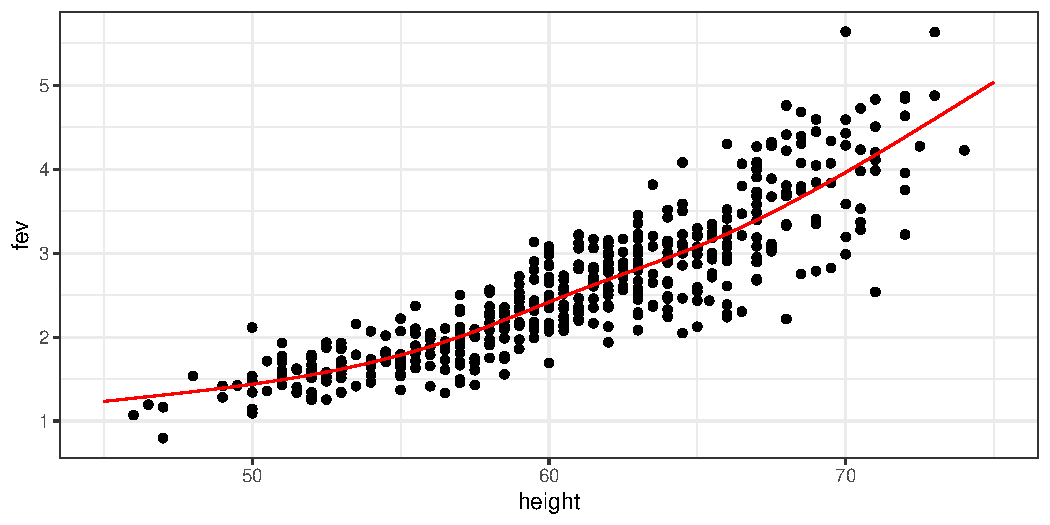
\includegraphics[width=\maxwidth]{figure/beamer-unnamed-chunk-5-1} 

}



\end{knitrout}




\end{frame}





%%%%%%%%%%%%%%%%%%%%%%%%%%%%%%%%%%%

\begin{frame}
\frametitle{What the numbers do not mean ...}

The most common mistake made when interpreting logistic regression is to treat an odds ratio as a ratio of probabilities.\\

~\\ 

Bird keepers are \emph{not} 4x more likely to develop lung cancer than non-bird keepers.

~\\ 

This is the difference between relative risk and an odds ratio.


\[RR = \frac{P(\text{disease} | \text{exposed})}{P(\text{disease} | \text{unexposed})} \]

\[OR = \frac{P(\text{disease} | \text{exposed}) / [1-P(\text{disease} | \text{exposed})]}{P(\text{disease} | \text{unexposed})/[1-P(\text{disease} | \text{unexposed})]} \]


\end{frame}


%%%%%%%%%%%%%%%%%%%%%%%%%%%%%%%%%%%

\begin{frame}[fragile]{Measuring accuracy of a model for binary outcomes}

A common metric for evaluating models for binary outcomes is simply called the ``accuracy''. 

It requires specifying a threshold ($c$) for the predicted probability ($\hat p_i$) that an individual has the outcome of interest. For a given threshold, we say that 
\[
    \hat y_i(c)= 
\begin{cases}
    1,    & \text{if }p_i \geq c\\
    0,  & \text{if } p_i < c\\ 
\end{cases}
\]

And then the accuracy, for a given $c$ is defined
$$ accuracy(c) = \sum_{i=1}^N \frac{1- | \hat y_i(c) - y_i | }{N} $$.

\end{frame}


%%%%%%%%%%%%%%%%%%%%%%%%%%%%%%%%%%%

\begin{frame}[fragile]{Measuring accuracy across all thresholds}

To gain a full picture of the accuracy of your model, you want to compute the accuracy for all possible values of $c$. This is what the ROC curve does:


\begin{knitrout}\scriptsize
\definecolor{shadecolor}{rgb}{0.969, 0.969, 0.969}\color{fgcolor}\begin{kframe}
\begin{alltt}
\hlkwd{library}\hlstd{(ROCR)}
\hlstd{birds}\hlopt{$}\hlstd{phat} \hlkwb{<-} \hlkwd{predict}\hlstd{(fm1,} \hlkwc{type}\hlstd{=}\hlstr{"response"}\hlstd{)}
\hlstd{pred} \hlkwb{<-} \hlkwd{prediction}\hlstd{(birds}\hlopt{$}\hlstd{phat, birds}\hlopt{$}\hlstd{LCnum)}
\hlstd{perf} \hlkwb{<-} \hlkwd{performance}\hlstd{(pred,}\hlstr{"tpr"}\hlstd{,}\hlstr{"fpr"}\hlstd{)}
\hlkwd{plot}\hlstd{(perf)}
\end{alltt}
\end{kframe}

{\centering 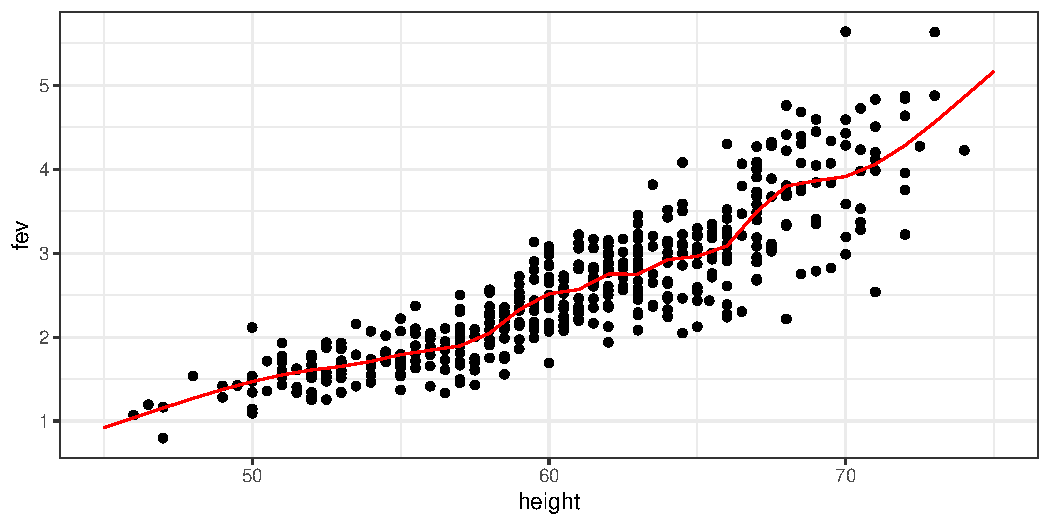
\includegraphics[width=\maxwidth]{figure/beamer-unnamed-chunk-6-1} 

}



\end{knitrout}



\end{frame}

%%%%%%%%%%%%%%%%%%%%%%%%%%%%%%%%%%%

\begin{frame}[fragile]{Measuring accuracy across all thresholds}

The "area under the curve" (AUC) is a common single measure of predictive accuracy of a model. It can be interpreted as {\em the probability, if one random individual with the outcome and one without were drawn from your dataset, that your model would accurately assign a higher $p_i$ to the one with the outcome.}

\begin{knitrout}\scriptsize
\definecolor{shadecolor}{rgb}{0.969, 0.969, 0.969}\color{fgcolor}\begin{kframe}
\begin{alltt}
\hlcom{## this prints out the computed area under the curve}
\hlkwd{performance}\hlstd{(pred,}\hlstr{"auc"}\hlstd{)}\hlopt{@}\hlkwc{y.values}
\end{alltt}
\begin{verbatim}
## [[1]]
## [1] 0.7746772
\end{verbatim}
\end{kframe}
\end{knitrout}


\begin{knitrout}\scriptsize
\definecolor{shadecolor}{rgb}{0.969, 0.969, 0.969}\color{fgcolor}

{\centering \includegraphics[width=\maxwidth]{figure/beamer-unnamed-chunk-8-1} 

}



\end{knitrout}



\end{frame}


%%%%%%%%%%%%%%%%%%%%%%%%%%%%%%%%%%%

% \begin{frame}[fragile]
% \frametitle{To match or not to match}
% 
% \begin{block}{Case-control studies are common for (rare) binary outcomes}
% \bi
%     \myitem Randomly selected controls $\longrightarrow$ vanilla logistic regression
%     \myitem Matched controls $\longrightarrow$ conditional logistic regression
% \ei
% \end{block}
% 
% \begin{block}{Conditional logistic regression}
% \bi
%     \myitem Accounts for the fact that you have ``adjusted'' for some variables in the design.
%     \myitem Calculates an OR for each matched-set/pair, then ``averages'' across sets
%     \myitem Forfeits ability to estimate effects of matched variables, but design can substantially improve power. 
%     \myitem Implemented in R with {\tt clogit()}.
% \ei
% \end{block}
% 
% \end{frame}


%%%%%%%%%%%%%%%%%%%%%%%%%%%%%%%%%%%

\begin{frame}[fragile]
\frametitle{Important notes about GLMs}

\begin{block}{On logistic regression in particular...}
\bi
        \myitem There are other link functions for binary data (e.g. probit, cloglog).
        \myitem Other, less parametric methods may be appropriate here too -- e.g. CART, random forests, classification algorithms.
\ei
\end{block}

\begin{block}{Beyond the scope of this course, but interesting topics...}
\bi
        \myitem How are logistic models (and other GLMs) fitted?
        \myitem Can we perform the same kind of model diagnostics to determine whether a model provides a good fit to data?
        \myitem Sensitivity and specificity
        \ei
\end{block}

\end{frame}

%%%%%%%%%%%%%%%%%%%%%%%%%%%%%%%%%%%

% \begin{frame}[fragile]{On your own...}
% 
% 
% \bi
%     \myitem Examine the residuals from the logistic regression model shown earlier with six predictors. Why does this plot look different than other residual plots we have seen this semester?
% <<eval=FALSE>>=
% plot(fm1, which=1)
% @
% 
%     \myitem A better way to look at residuals for logistic regression is using "binned residual plots". Divide your observations into bins with equal numbers of observations along some variable of interest (e.g. the fitted values, or one of your covariates). Then, calculate the average residual in that bin. Luckily, there is a function that can do this for us! 
% <<eval=FALSE>>=
% library(arm)
% binnedplot(birds$AG, resid(fm1), nclass=20)
% @
% 
% Evaluate binned residual plots across continuous predictor variables as well as the ``fitted'' model values. Do you see any violations of the assumption that the mean residual is far away from zero?
% 
% 
% \ei
% 
% \end{frame}

%%%%%%%%%%%%%%%%%%%%%%%%%%%%%%%%%%%

\begin{frame}[fragile]


\centering
\Large
Mathematical details


\end{frame}

%%%%%%%%%%%%%%%%%%%%%%%%%%%%%%%%%%%

\begin{frame}[fragile]
\frametitle{Generalized linear models: defined}

All generalized linear models have the following three characteristics:
\begin{enumerate}
\item {\bf A probability distribution} describing the outcome variable \\
\bi
\item e.g. $Y \sim \text{Bernoulli}(p) \longrightarrow \mathbb E[Y|p] = p$. 
\ei
\item {\bf A linear model}
\begin{itemize}
\item $\eta = \beta_0+\beta_1 X_1 + \cdots + \beta_p X_p$
\end{itemize}
\item {\bf A link function} that relates the linear model to the parameter of the outcome distribution
\begin{itemize}
\item $g(\mathbb E[Y]) = g(p) = \eta$ or $\mathbb E[Y] = p = g^{-1}(\eta)$
\end{itemize}
\end{enumerate}

\end{frame}


%%%%%%%%%%%%%%%%%%%%%%%%%%%%%%%%%%%

\begin{frame}
\frametitle{MLR is a special case of a GLM}

\begin{block}{For continuous outcome, we often do this}
\begin{enumerate}
\item {\bf A probability distribution} describing the outcome variable \\
\bi
\item $Y|X \sim \text{Normal}(\mu, \sigma^2) \longrightarrow \mathbb E[Y|X] = \mu$. 
\ei
\item {\bf A linear model}
\begin{itemize}
\item $\eta = \beta_0+\beta_1 X_1 + \cdots + \beta_p X_p$
\end{itemize}
\item {\bf A link function} that relates the linear model to the parameter of the outcome distribution
\begin{itemize}
\item $g(\mathbb E[Y|X]) = g(\mu) = \mu = \eta$ 
\end{itemize}
\end{enumerate}
\end{block}

$$g(\mathbb E[Y|X]) = E[Y|X] = \mu = \beta_0+\beta_1 X_1 + \cdots + \beta_p X_p$$

\end{frame}


%%%%%%%%%%%%%%%%%%%%%%%%%%%%%%%%%%%

\begin{frame}
\frametitle{Logistic regression: a common GLM for 0/1 outcome data}

\begin{enumerate}
\item {\bf A probability distribution} describing the outcome variable \\
\bi
\item $Y|X \sim \text{Bernoulli}(p) \longrightarrow \mathbb E[Y|X] = Pr(Y=1|X) = p$. 
\ei
\item {\bf A linear model}
\begin{itemize}
\item $\eta = \beta_0+\beta_1 X_1 + \cdots + \beta_p X_p$
\end{itemize}
\item {\bf A link function} that relates the linear model to the parameter of the outcome distribution
\begin{itemize}
\item $g(\mathbb E[Y|X]) = g(p) = logit(p) = \log\frac{p}{1-p} = \eta$ 
\end{itemize}
\end{enumerate}

$$g(\mathbb E[Y|X]) = logit[Pr(Y=1|X)] = \beta_0+\beta_1 X_1 + \cdots + \beta_p X_p$$

\end{frame}




\end{document}
